% MATLAB source: paper/plot_existing_manuscript_figures.m
\begin{figure}[tbp]
  \centering
  \begin{subfigure}[t]{0.485\linewidth}
    \centering
    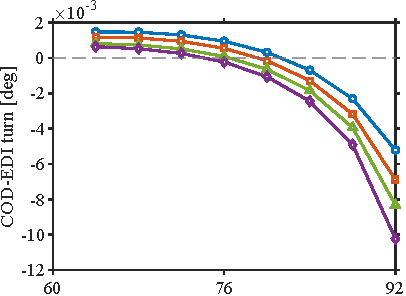
\includegraphics[width=\linewidth]{figures/cod/turn_linear.pdf}
    \caption{Turning-angle differences for linear COD fits.}
    \label{fig:cod-turn-linear}
  \end{subfigure}
  \hfill
  \begin{subfigure}[t]{0.485\linewidth}
    \centering
    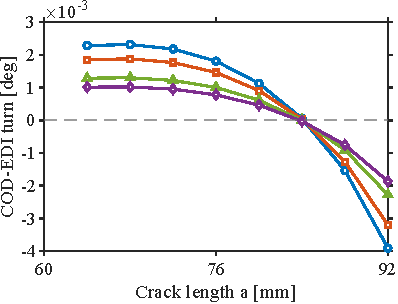
\includegraphics[width=\linewidth]{figures/cod/turn_quadratic.pdf}
    \caption{Turning-angle differences for quadratic COD fits.}
    \label{fig:cod-turn-quadratic}
  \end{subfigure}

  \medskip

  \begin{subfigure}[t]{0.485\linewidth}
    \centering
    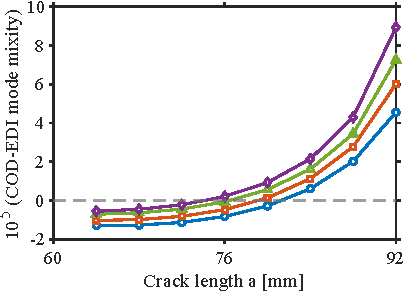
\includegraphics[width=\linewidth]{figures/cod/mixity_linear.pdf}
    \caption{Mode-mixity differences for linear COD fits.}
    \label{fig:cod-mixity-linear}
  \end{subfigure}
  \hfill
  \begin{subfigure}[t]{0.485\linewidth}
    \centering
    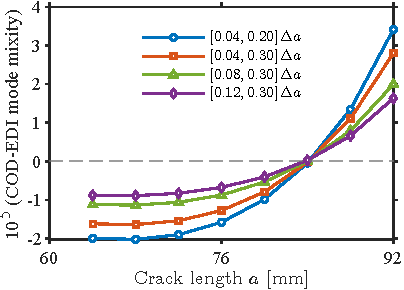
\includegraphics[width=\linewidth]{figures/cod/mixity_quadratic.pdf}
    \caption{Mode-mixity differences for quadratic COD fits.}
    \label{fig:cod-mixity-quadratic}
  \end{subfigure}

  \caption{Late-path extraction differences for all four native COD windows
  and both polynomial degrees. Window bounds are multiples of $\Delta a$.
  Zero is equality with EDI, not a known exact solution. The upper panels
  show differences in the MTS turns computed from the two sets of SIFs;
  the lower panels show differences in mode mixity. The largest observed
  difference occurs at the last accepted tip; individual difference curves
  need not vary monotonically.}
  \label{fig:cod}
\end{figure}
